%%%%%%%%%%%%%%%%%%%%%%%%%%%%%%%%%%%%%%%%%
% University Assignment Title Page
% LaTeX Template
% Version 1.0 (27/12/12)
%
% This template has been downloaded from:
% http://www.LaTeXTemplates.com
%
% Original author:
% WikiBooks (http://en.wikibooks.org/wiki/LaTeX/Title_Creation)
%
% License:
% CC BY-NC-SA 3.0 (http://creativecommons.org/licenses/by-nc-sa/3.0/)
%
% Instructions for using this template:
% This title page is capable of being compiled as is. This is not useful for
% including it in another document. To do this, you have two options:
%
% 1) Copy/paste everything between \begin{document} and \end{document}
% starting at \begin{titlepage} and paste this into another LaTeX file where you
% want your title page.
% OR
% 2) Remove everything outside the \begin{titlepage} and \end{titlepage} and
% move this file to the same directory as the LaTeX file you wish to add it to.
% Then add \input{./title_page_1.tex} to your LaTeX file where you want your
% title page.
%
%%%%%%%%%%%%%%%%%%%%%%%%%%%%%%%%%%%%%%%%%
%\title{Title page with logo}
%----------------------------------------------------------------------------------------
%   PACKAGES AND OTHER DOCUMENT CONFIGURATIONS
%----------------------------------------------------------------------------------------

\documentclass[12pt]{article}
\usepackage[english]{babel}

\usepackage{float}
% \usepackage{subfig}
\usepackage{wrapfig}
\usepackage[utf8]{inputenc}
\usepackage[top=1in, bottom=1in, left=1.25in, right=1.25in]{geometry}
\usepackage{amsmath}
\usepackage[toc,page]{appendix}
\usepackage{graphicx}
\usepackage{listings}
\usepackage{cleveref}
\usepackage{listings}
\usepackage{listingsutf8}
\usepackage{ucs}
\usepackage[affil-it]{authblk}
\graphicspath{ {figures/}}
\usepackage[colorinlistoftodos]{todonotes}
\lstset{numbers=none,
numberstyle=\tiny,
keywordstyle=\color{blue!70}, commentstyle=\color{red!50!green!50!blue!50},
frame=single,inputencoding=utf8x,
rulesepcolor=\color{red!20!green!20!blue!20},
breaklines=true,basicstyle=\scriptsize
}



\begin{document}

\begin{titlepage}

\newcommand{\HRule}{\rule{\linewidth}{0.5mm}} % Defines a new command for the horizontal lines, change thickness here

\center % Center everything on the page

%----------------------------------------------------------------------------------------
%   HEADING SECTIONS
%----------------------------------------------------------------------------------------

\textsc{\LARGE University of California, Davis}\\[1cm] % Name of your university/college
\textsc{\Large Department of Land, Air and Water}\\[0.5cm] % Major heading such as course name
% \textsc{\large Minor Heading}\\[0.5cm] % Minor heading such as course title

%----------------------------------------------------------------------------------------
%   TITLE SECTION
%----------------------------------------------------------------------------------------

\HRule \\[0.4cm]
{ \huge \bfseries Field Data-logger 1.0}\\[0.4cm] % Title of your document
\HRule \\[1cm]

%----------------------------------------------------------------------------------------
%   AUTHOR SECTION
%----------------------------------------------------------------------------------------

% \begin{minipage}{0.4\textwidth}
% \begin{flushleft} \large
% \emph{Members:}\\
% Hengjiu \textsc{Kang}   \\ % Your name  \\
% \end{flushleft}
% \end{minipage}
% ~
% \begin{minipage}{0.4\textwidth}
% \begin{flushright} \large
% \emph{Supervisor:} \\
% Dr. Andre \textsc{Knoesen} % Supervisor's Name
% \end{flushright}
% \end{minipage}\\[2cm]

% If you don't want a supervisor, uncomment the two lines below and remove the section above
\Large \emph{Author:}\\
Hengjiu \textsc{Kang}\\[3cm] % Your name

%----------------------------------------------------------------------------------------
%   DATE SECTION
%----------------------------------------------------------------------------------------

{\large \today}\\[1.5cm] % Date, change the \today to a set date if you want to be precise

%----------------------------------------------------------------------------------------
%   LOGO SECTION
%----------------------------------------------------------------------------------------

% 
\includegraphics[scale=0.5]{uc-davis.png}\\[1cm] % Include a department/university logo - this will require the graphicx package

%----------------------------------------------------------------------------------------

\vfill % Fill the rest of the page with whitespace

\end{titlepage}

\author{Hengjiu Kang%
  \thanks{Electronic address: \texttt{hjkang@ucdavis.edu}}}
\affil{Department of Electrical and Computer Engineering, University of California, Davis}


\title{Field Data-Loger 1.0}
\maketitle

\newpage
\begin{figure}[H]
\centering
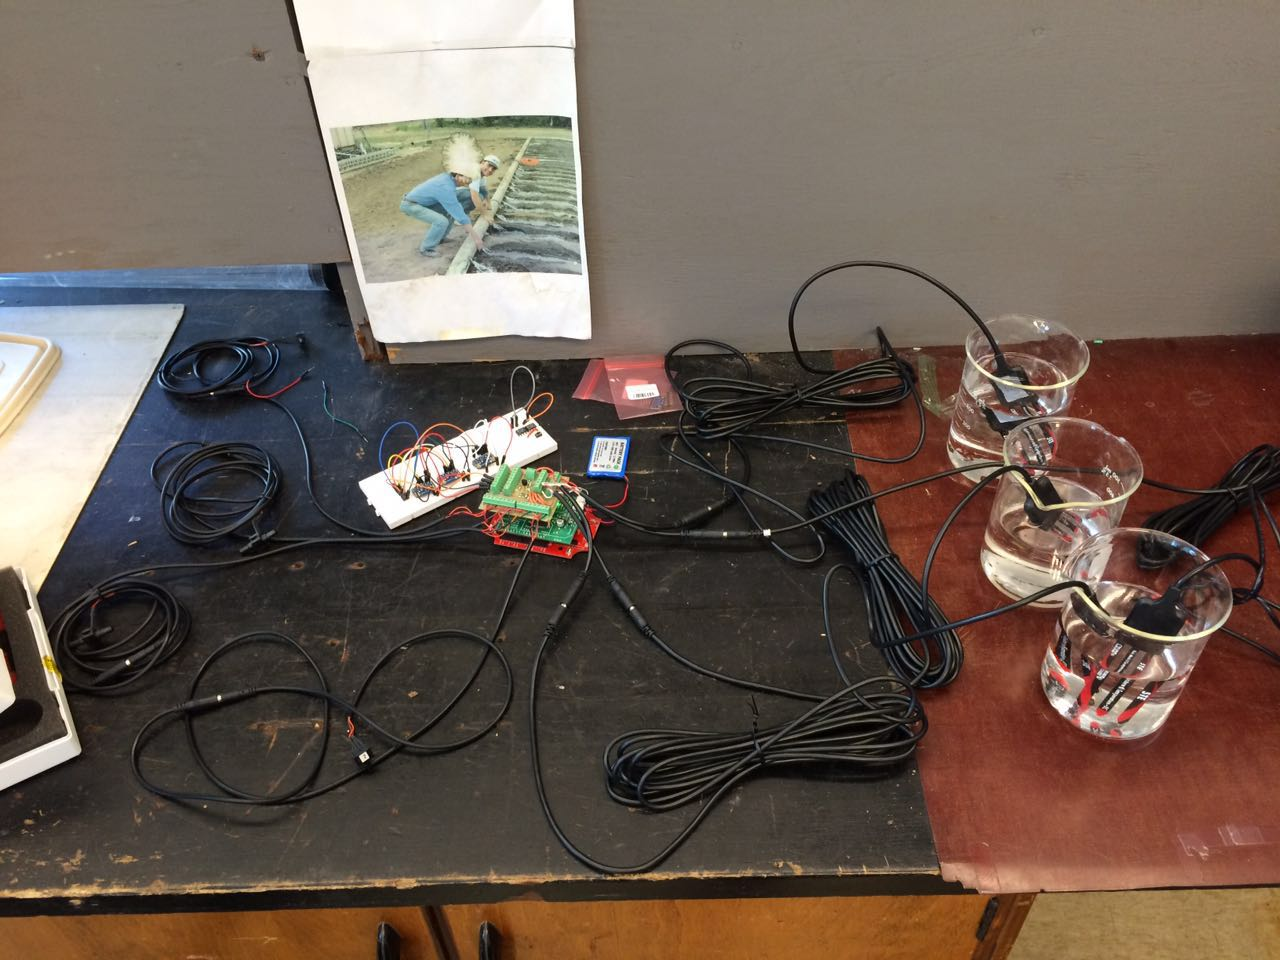
\includegraphics[width=\textwidth]{overall.jpg}
\caption{\emph{Overall view of field Data-logger}}
\end{figure}

\newpage
\tableofcontents \newpage
\listoffigures  \newpage

\newpage

\section{Overview}
    This Field Data-logger is a new hardware based on Atmega328 chip which fuses multiple type of sensors from different brands. It can collect data in programmable period of time, and thanks to low power design, this Field Data-logger can last for very long time when solar panel is installed.

\section{Features}
    \begin{itemize}
    \item 8 16-bit single ended or 4 16-bit differential ADC inputs
    \item 4 $I^{2}C$ connection ports
    \item 4 Read only sensors inputs
    \item Programmable wake up RTC
    \item Solar panel
    \item On-board SD card
    \item XBee network (Will be available in the next version)
    \end{itemize}


\newpage
\section{Hardware Design}
  \subsection{Absolut values}
    \subsection{Electrical Systems}
            \begin{figure}[ht]
            \centering
            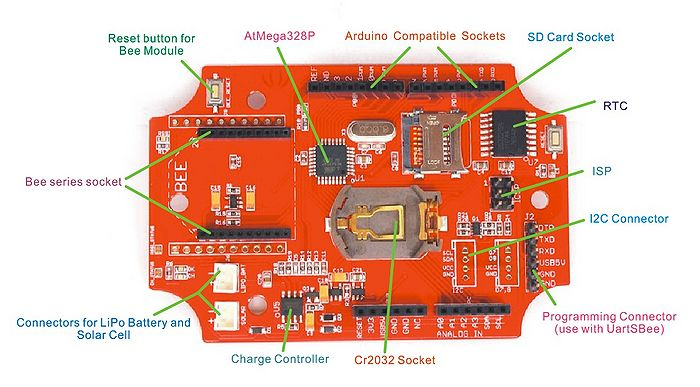
\includegraphics[width=0.9\textwidth]{Stalker.jpg}
            \caption{\label{fig:Seeeduino Stalker}Seeeduino Stalker v2.3}
            \end{figure}
    Arduino Based controller 
    \subsection{Power distribution}
    \subsection{RTC}
    \subsection{$I^{2}C$}
    \subsection{ADC}
    \subsection{Read-Only Port}

    
           

\newpage
\section{Software Design}


    \subsection{Overall strucutre}
    All the components in this robot are written in C++ 11 with STL and Linux components for speed consideration. The operations 
% \newpage
\section{Results}
    \subsection{Design achivement}
       

% \newpage
\section{Future Work}




\newpage
\section{Acknowledgements and References}
\begin{thebibliography}{9}

\bibitem{ExploringBBB}
  Derek Molloy,
  \emph{Exploring Beaglebone},
  Wiley, Hoboken,
  1nd edition,
  2014.

\bibitem{PIDTuning}
  Sigurd Skogestad,
  \emph{Probaly the best simple PID tuning rules in the world},
  Department of Chemical Engineering,
  Norwegian University of Science and Technology,
  2001.

\bibitem{Kalman}
  Greg Welch, Grary Bishop,
  \emph{An Introduction to the Kalman Filter},
  Department of Computer Science,
  University of North Carolina at Chapel Hill,
  Chapel Hill, NC.

\bibitem{deviceTree}
  Justin Cooper,
  \emph{Introduction to the BeagleBone Black Device Tree},
  Adafruit,
  https://learn.adafruit.com/introduction-to-the-beaglebone-black-device-tree/overview,
  2014.

\bibitem{KalmanLib}
  Kristian Lauszus,
  \emph{KalmanFilter},
  TKJ Electronics 2012,
  https://github.com/TKJElectronics/KalmanFilter,
  2012.

\bibitem{Blacklib}
  Yiğit Yüce,
  \emph{Black Lib},
  http://blacklib.yigityuce.com/.

\bibitem{hackinWiiCamera}
  Eric Jacob,
  \emph{Wii Remote IR Camera Hack with Arduino Interface},
  http://www.instructables.com/id/Wii-Remote-IR-Camera-Hack/,
  2010.

\end{thebibliography}

\renewcommand{\abstractname}{Acknowledgements}
\begin{abstract}
Special thanks to Bay Area Circuit
\end{abstract}
\renewcommand{\abstractname}{Abstract}

\begin{appendices}
    \section{Mechanical Design}
        \subsection{Mechanical Design}
            \label{sw:structure}

            


    \section{PCB Design}
        \subsection{Shield}
           
        \subsection{Ankle Band}
            \label{ad:band}
            \begin{figure}[H]
            \centering
            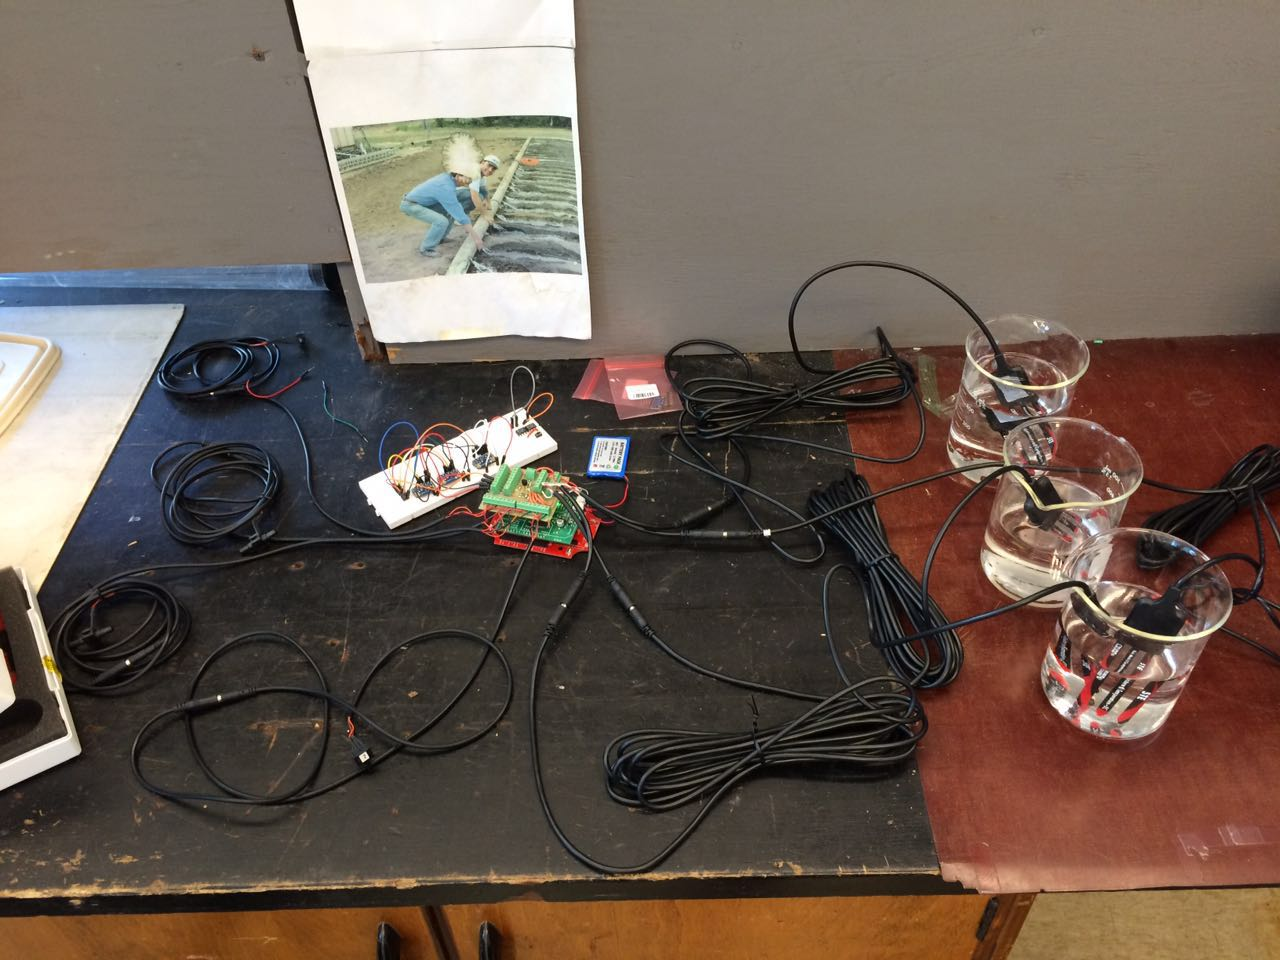
\includegraphics[width=0.2\textwidth]{overall.jpg}
            \caption{\label{fig:band_layout}Unpoured Band PCB Layout}
            \end{figure}

    \section{BOM}
    Due to limited space, please check individual BOM file.

    \section{Source code}
        \subsection{Applications}
            \label{source:applications}
            \subsubsection{Main on Beaglebone Black}
                \lstinputlisting[language=C++]{src/IRAssemblyTest/main.cpp}
            \subsubsection{IMU on Arduino}
                \lstinputlisting[language=C++]{src/imu/kalmanSPI.ino}
            \subsubsection{IMU on Beaglebone Black}
                \lstinputlisting[language=C++]{src/arduinoConnector/arduinoConnector.cpp}
                \lstinputlisting[language=C++]{src/arduinoConnector/arduinoConnector.h}

        \subsection{Libries}
            \label{source:libs}
            \subsubsection{Customized Libs}
                \lstinputlisting[language=C++]{src/BlackServo/BlackServo.h}
                \lstinputlisting[language=C++]{src/BlackStepper/BlackStepper.h}
                \lstinputlisting[language=C++]{src/BlackStepper/DualStepperMotor.h}
            \subsubsection{IR Camera Driver}
                \lstinputlisting[language=C++]{src/PVision/BlobCompare.h}
                \lstinputlisting[language=C++]{src/PVision/IR_target.h}
                \lstinputlisting[language=C++]{src/PVision/IRRim.h}
                \lstinputlisting[language=C++]{src/PVision/PCA9548A.h}
                \lstinputlisting[language=C++]{src/PVision/PVision.h}
                \lstinputlisting[language=C++]{src/PVision/proximityRing.h}
                \lstinputlisting[language=C++]{src/PVision/vec.h}
            \subsubsection{PID control}
                \lstinputlisting[language=C++]{src/PID/PID.h}
        \subsection{Device tree}
            \label{source:overlays}
            \lstinputlisting{src/overlay/bspm_P9_25_17-00A0.dts}
            \lstinputlisting{src/overlay/bspwm_P9_29_11-00A0.dts}
            \lstinputlisting{src/overlay/bspwm_P9_31_11-00A0.dts}
    \section{User Manual}
\end{appendices}


% \todo {parts following are for referencing, because Im not familiar with latex}
% \subsection{Tables and Figures}

% Use the table and tabular commands for basic tables --- see Table~\ref{tab:widgets}, for example. You can upload a figure (JPEG, PNG or PDF) using the files menu. To include it in your document, use the includegraphics command as in the code for Figure~\ref{fig:frog} below.

% % Commands to include a figure:
% \begin{figure}
% \centering
% \includegraphics[width=0.5\textwidth]{frog.jpg}
% \caption{\label{fig:frog}This is a figure caption.}
% \end{figure}

% \begin{table}
% \centering
% \begin{tabular}{l|r}
% Item & Quantity \\\hline
% Widgets & 42 \\
% Gadgets & 13
% \end{tabular}
% \caption{\label{tab:widgets}An example table.}
% \end{table}

% \subsection{Mathematics}

% \LaTeX{} is great at typesetting mathematics. Let $X_1, X_2, \ldots, X_n$ be a sequence of independent and identically distributed random variables with $\text{E}[X_i] = \mu$ and $\text{Var}[X_i] = \sigma^2 < \infty$, and let
% $$S_n = \frac{X_1 + X_2 + \cdots + X_n}{n}
%       = \frac{1}{n}\sum_{i}^{n} X_i$$
% denote their mean. Then as $n$ approaches infinity, the random variables $\sqrt{n}(S_n - \mu)$ converge in distribution to a normal $\mathcal{N}(0, \sigma^2)$.

% \subsection{Lists}

% You can make lists with automatic numbering \dots

% \begin{enumerate}
% \item Like this,
% \item and like this.
% \end{enumerate}
% \dots or bullet points \dots
% \begin{itemize}
% \item Like this,
% \item and like this.
% \end{itemize}

% We hope you find write\LaTeX\ useful, and please let us know if you have any feedback using the help menu above.

\end{document}